\chapter{结果检验}
\label{cha:results}

\section{网站介绍}
\label{chap:website-intro}

\subsection{展示全部可能有漏洞的主机功能}
\label{sec:show-all}

本系统最终的呈现方式是一个网站,具有展示可能具有漏洞的主机和相应的搜索功能。图~\ref{fig:main-page}是网站的首页,也是能够展示全部可能具有高危漏洞的主机的地方。
在此例中,监测的主机范围是166.111.0.0/16,监测的CVE范围是全部2018年的CVE。

\begin{figure}[H]
    \centering
    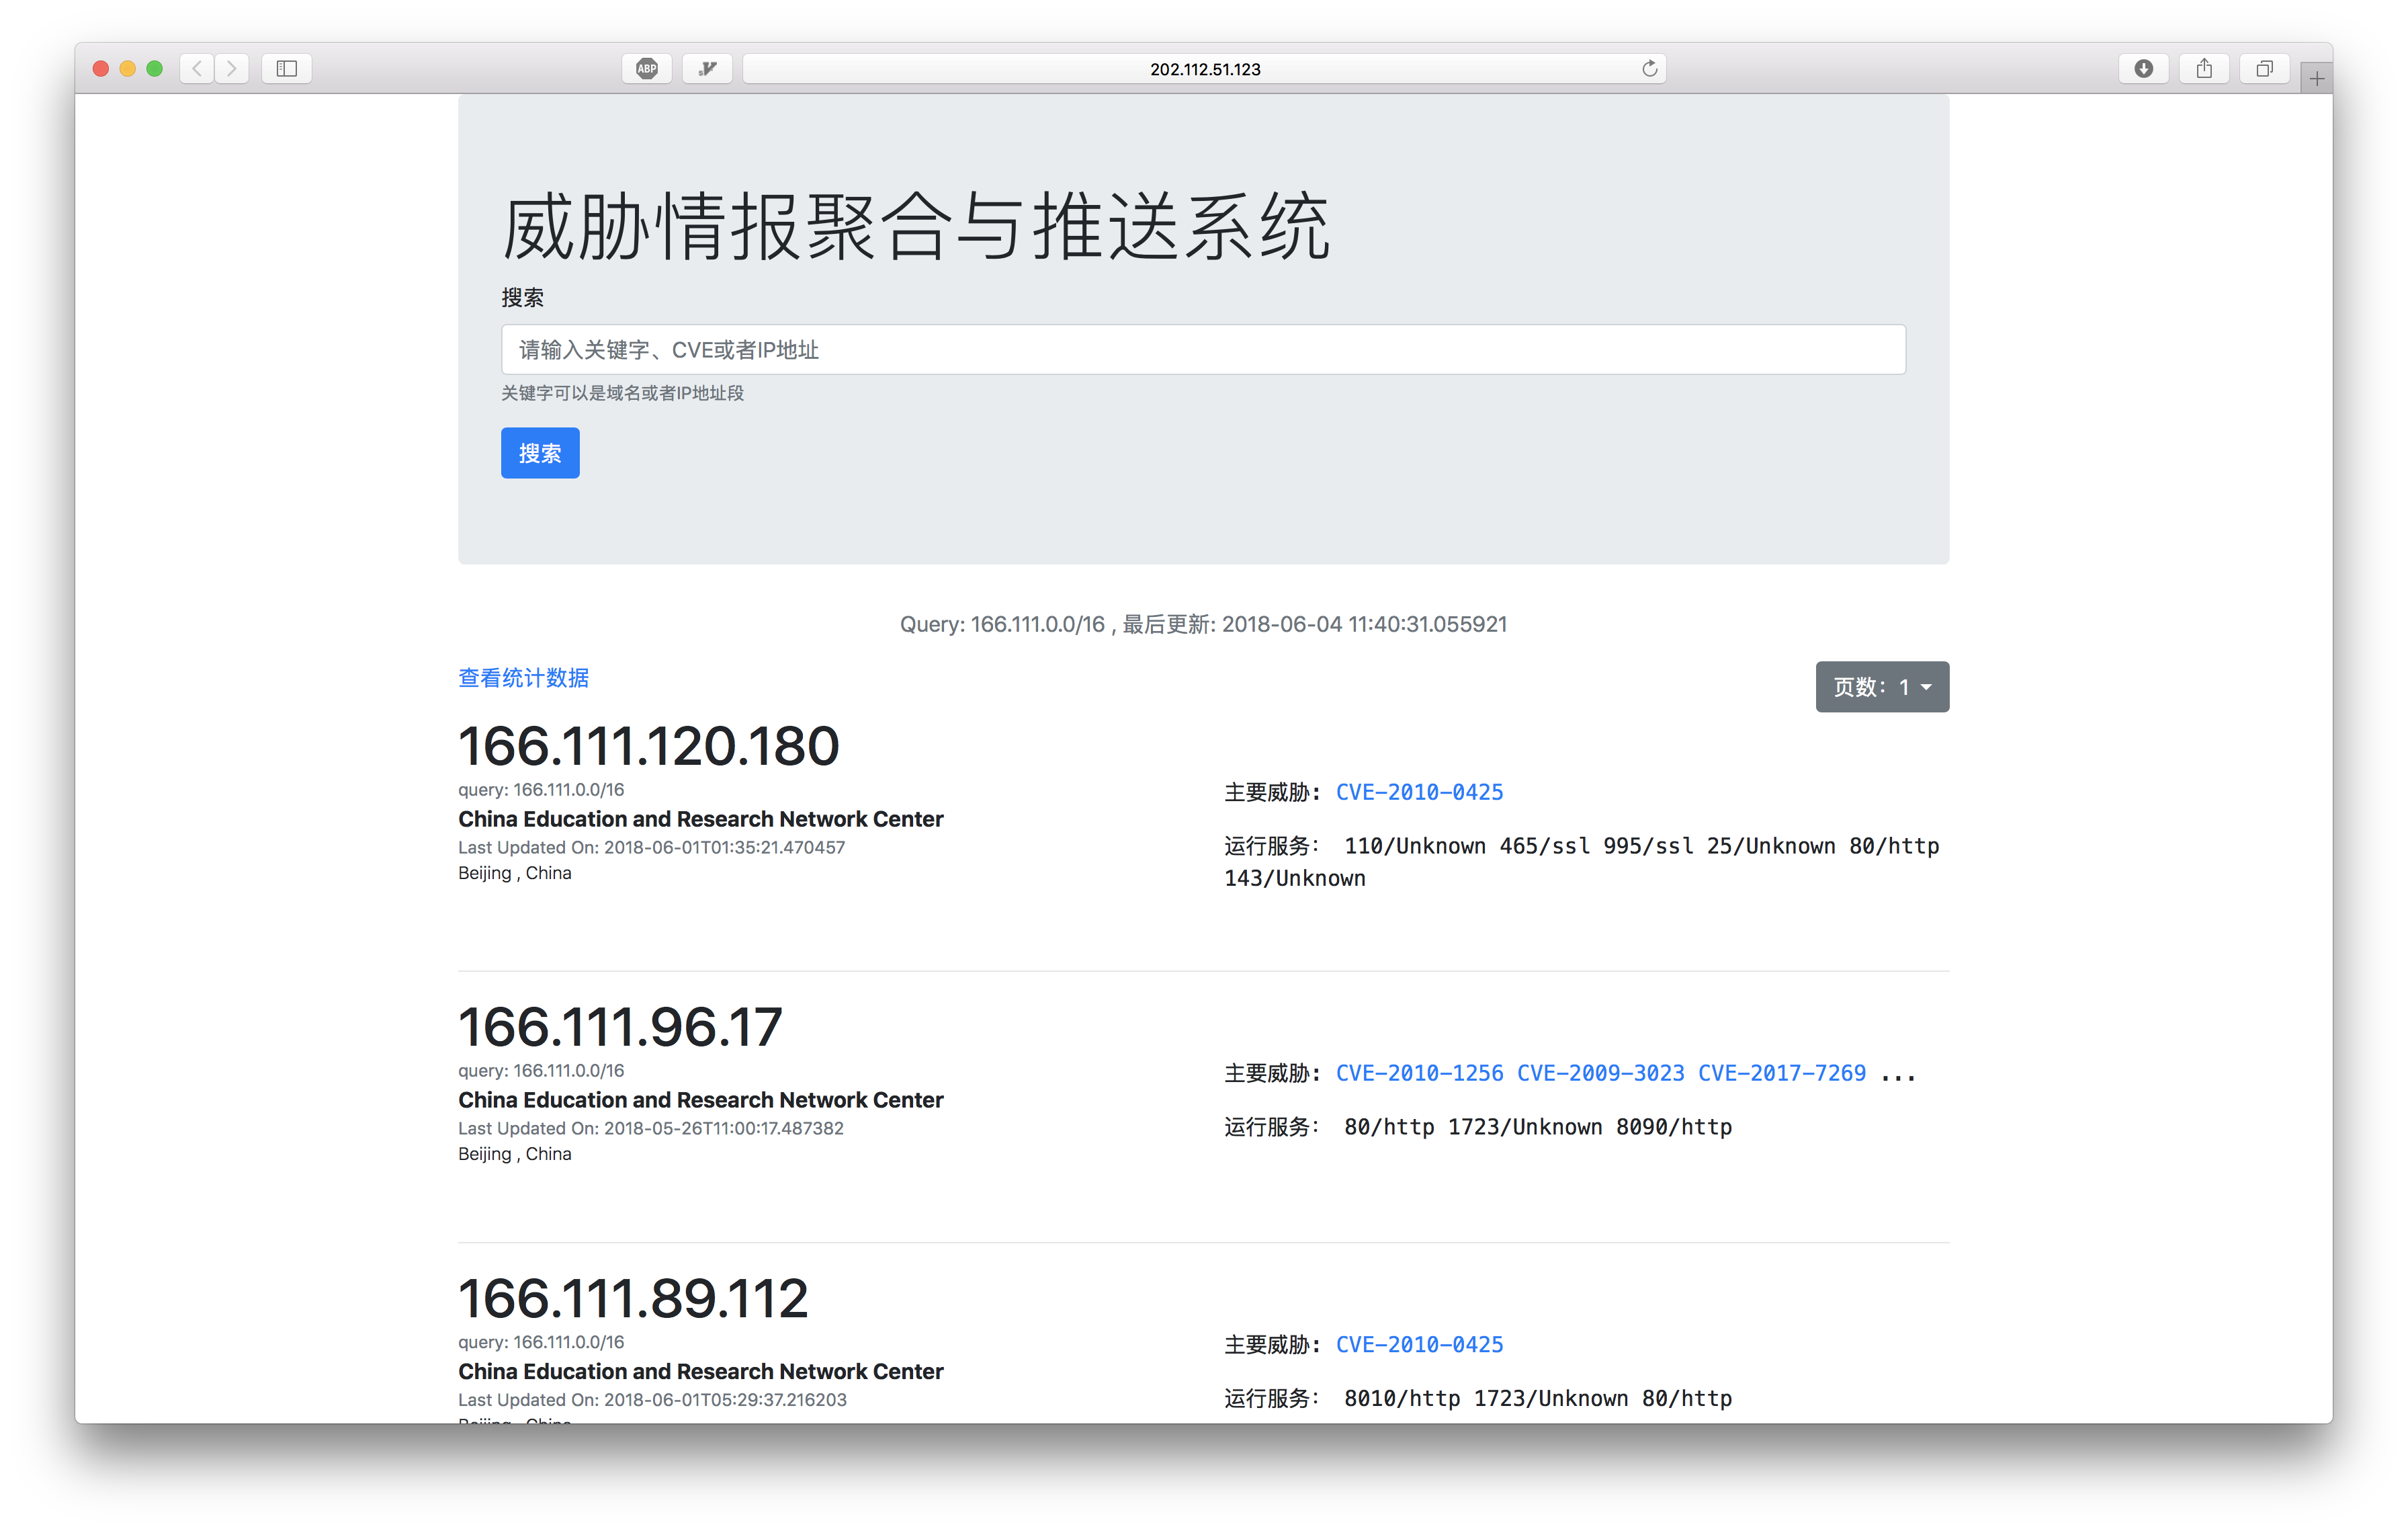
\includegraphics[scale=0.12]{main-page.png}
    \caption{网站主页}
    \label{fig:main-page}
\end{figure}

可以看到,网站的主要部分是一个列表,这列表里面的主机都可能存在高危漏洞,也即CVSS评分至少为8的CVE。每一个项目的左侧是主机的基本信息,
右侧显示了主要的威胁和运行的服务。点击IP地址可以进入主机的详情页面,点击CVE可以进入该CVE的详情页面。

在右侧有一个能够进行页面跳转的按钮,可以选择当前显示第几页的内容,因为1页最多显示10条。

\subsection{主机详情功能}
\label{sec:details}

在点击主页上的主机的IP地址之后可以进入该主机的详情界面,图~\ref{fig:details}展示了其中一台IP地址为166.111.68.30主机的详情。

\begin{figure}[H]
    \centering
    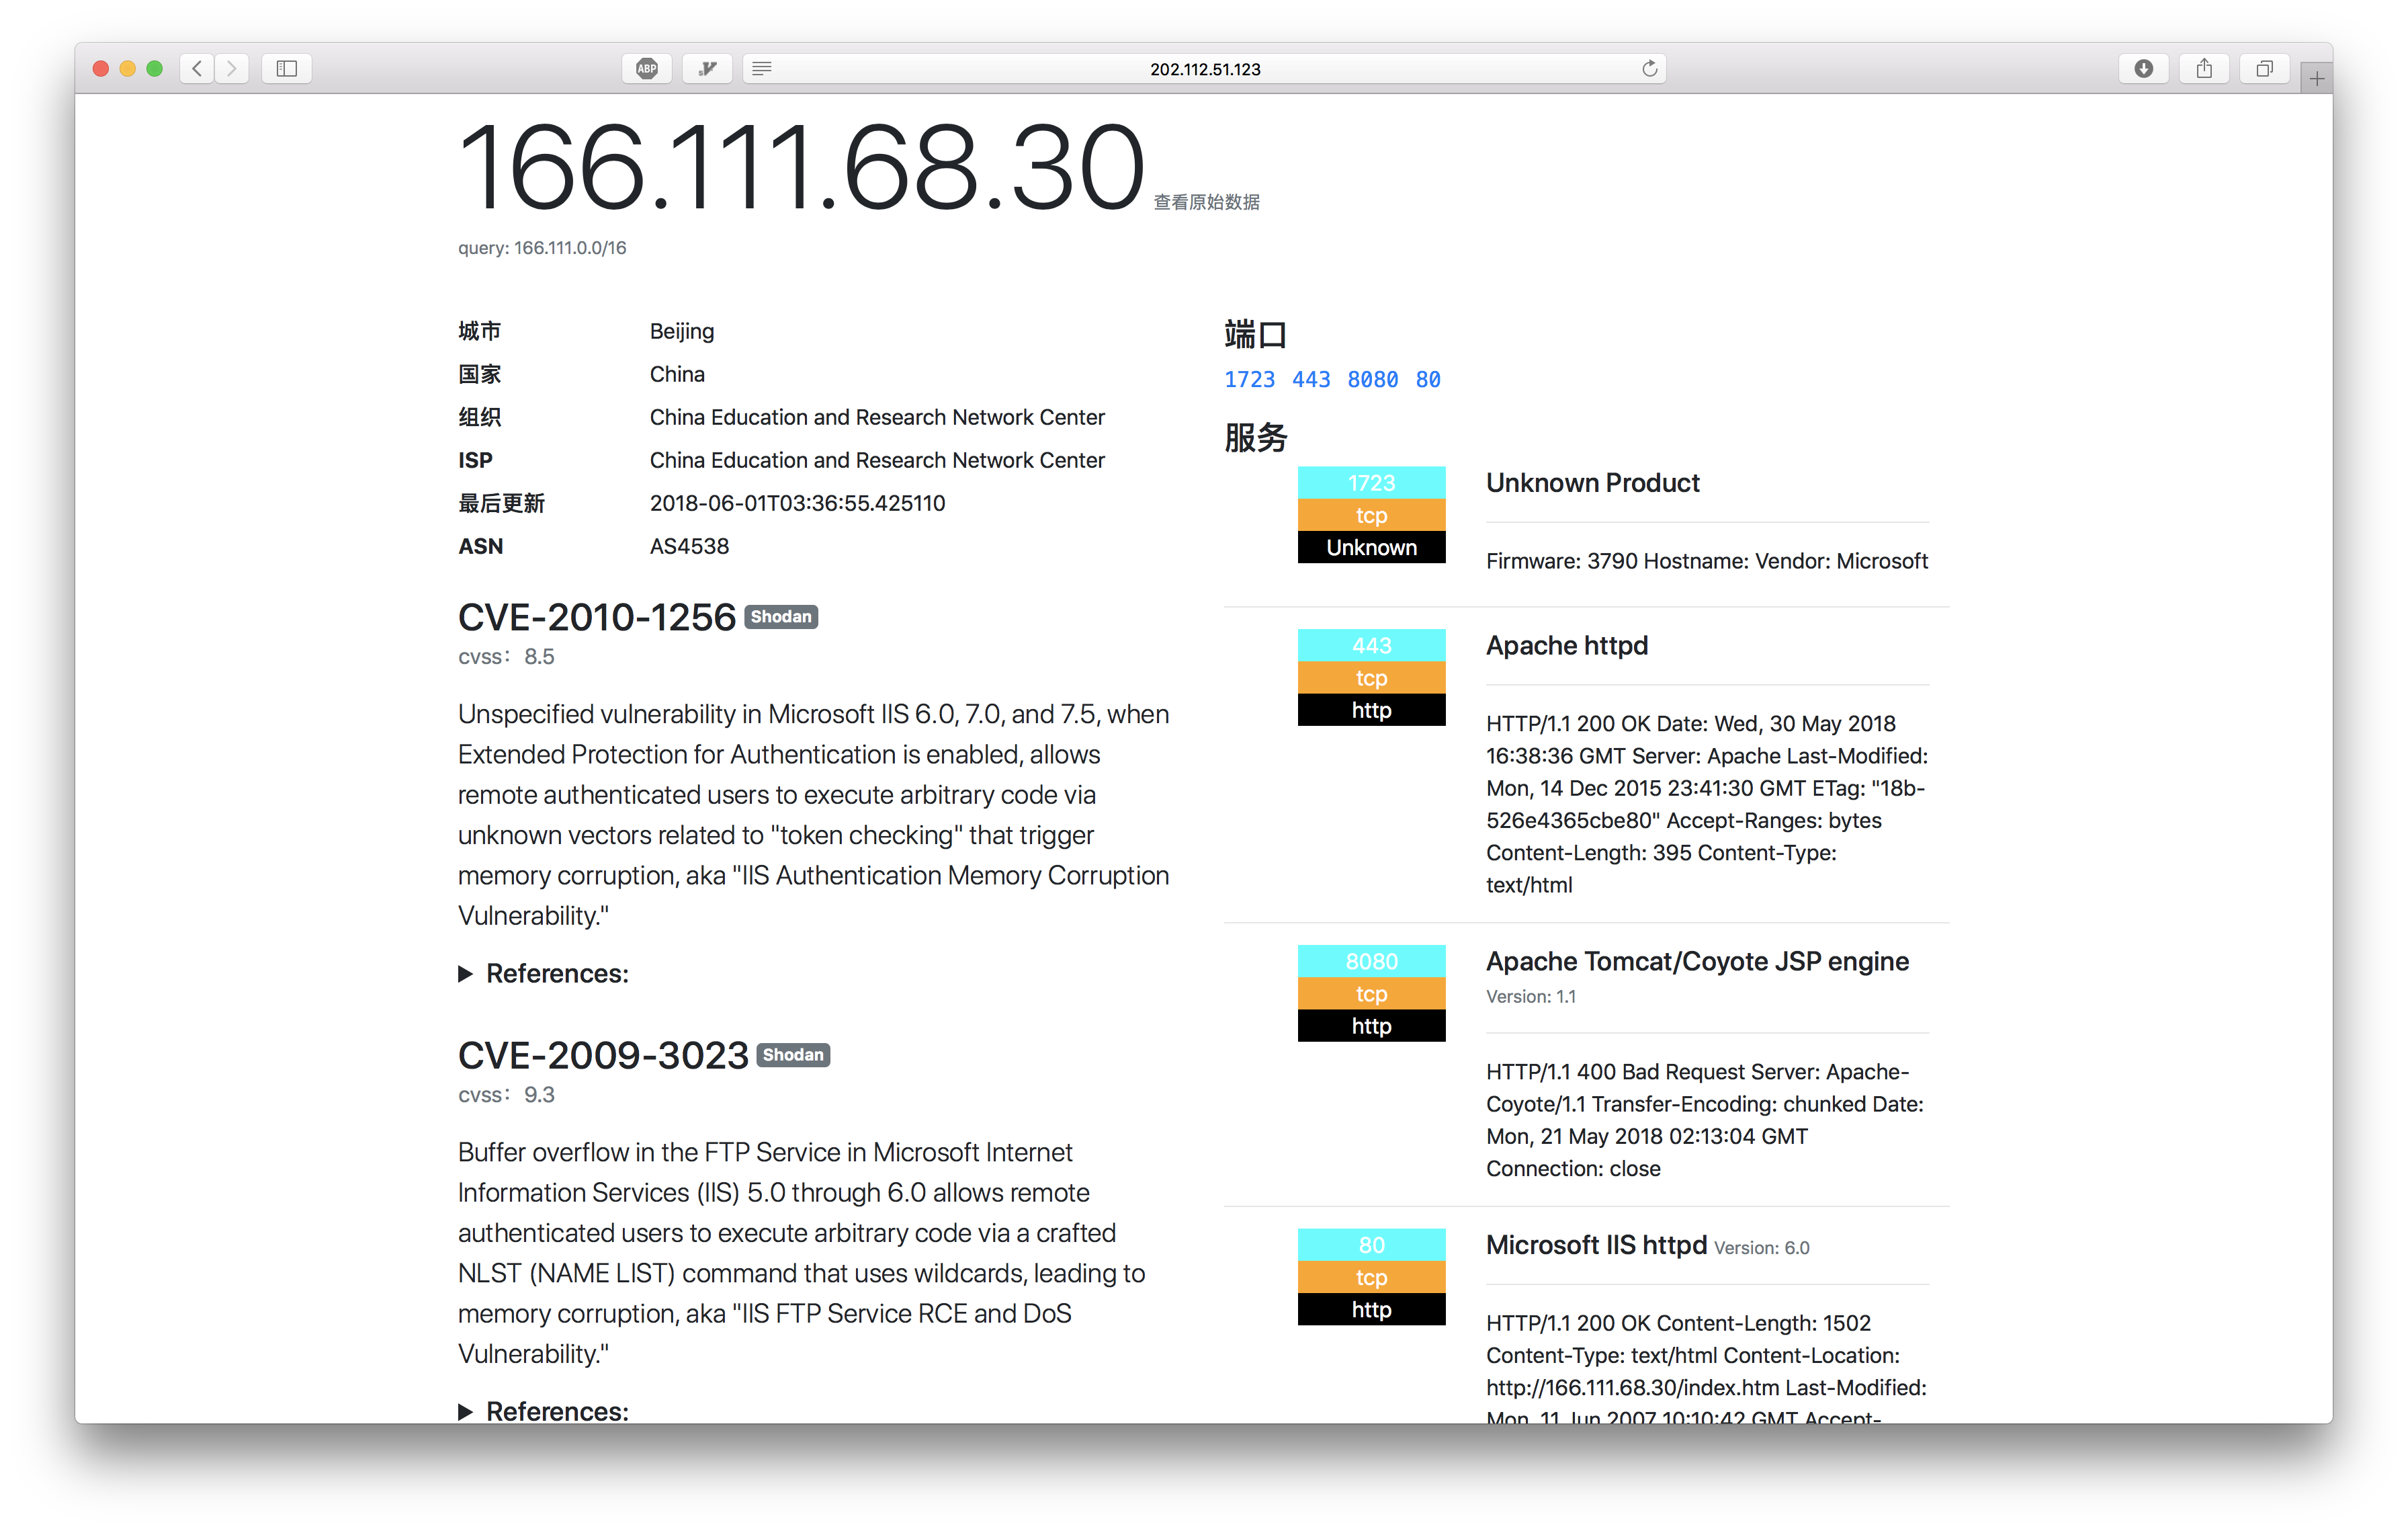
\includegraphics[scale=0.12]{details.png}
    \caption{主机详情界面}
    \label{fig:details}
\end{figure}

在该界面,可以看到该主机的基本信息,可能受到威胁的CVE以及对应的详细信息,这里提供了简介、CVSS评分、相关阅读等功能,
还能看到该主机开放的端口和运行的服务和其上运行的软件。点击IP地址旁边的查看原始数据还能看到原始json格式的主机信息。

\subsection{搜索功能}
\label{sec:search}

在首页的搜索栏里输入相应关键词可以进行一些简单的搜索,比如搜索IP地址、CVE名称或者Query的名称。图~\ref{fig:search}是搜索关键词“CVE-2018-0171”的结果,
显示了一台可能受到该CVE威胁的主机。

在图中可以看出,该主机的IP地址为166.111.176.55,是监测的范围166.111.0.0/16中的一台,右侧的CVE被染红表示这是关键词。

\begin{figure}[H]
    \centering
    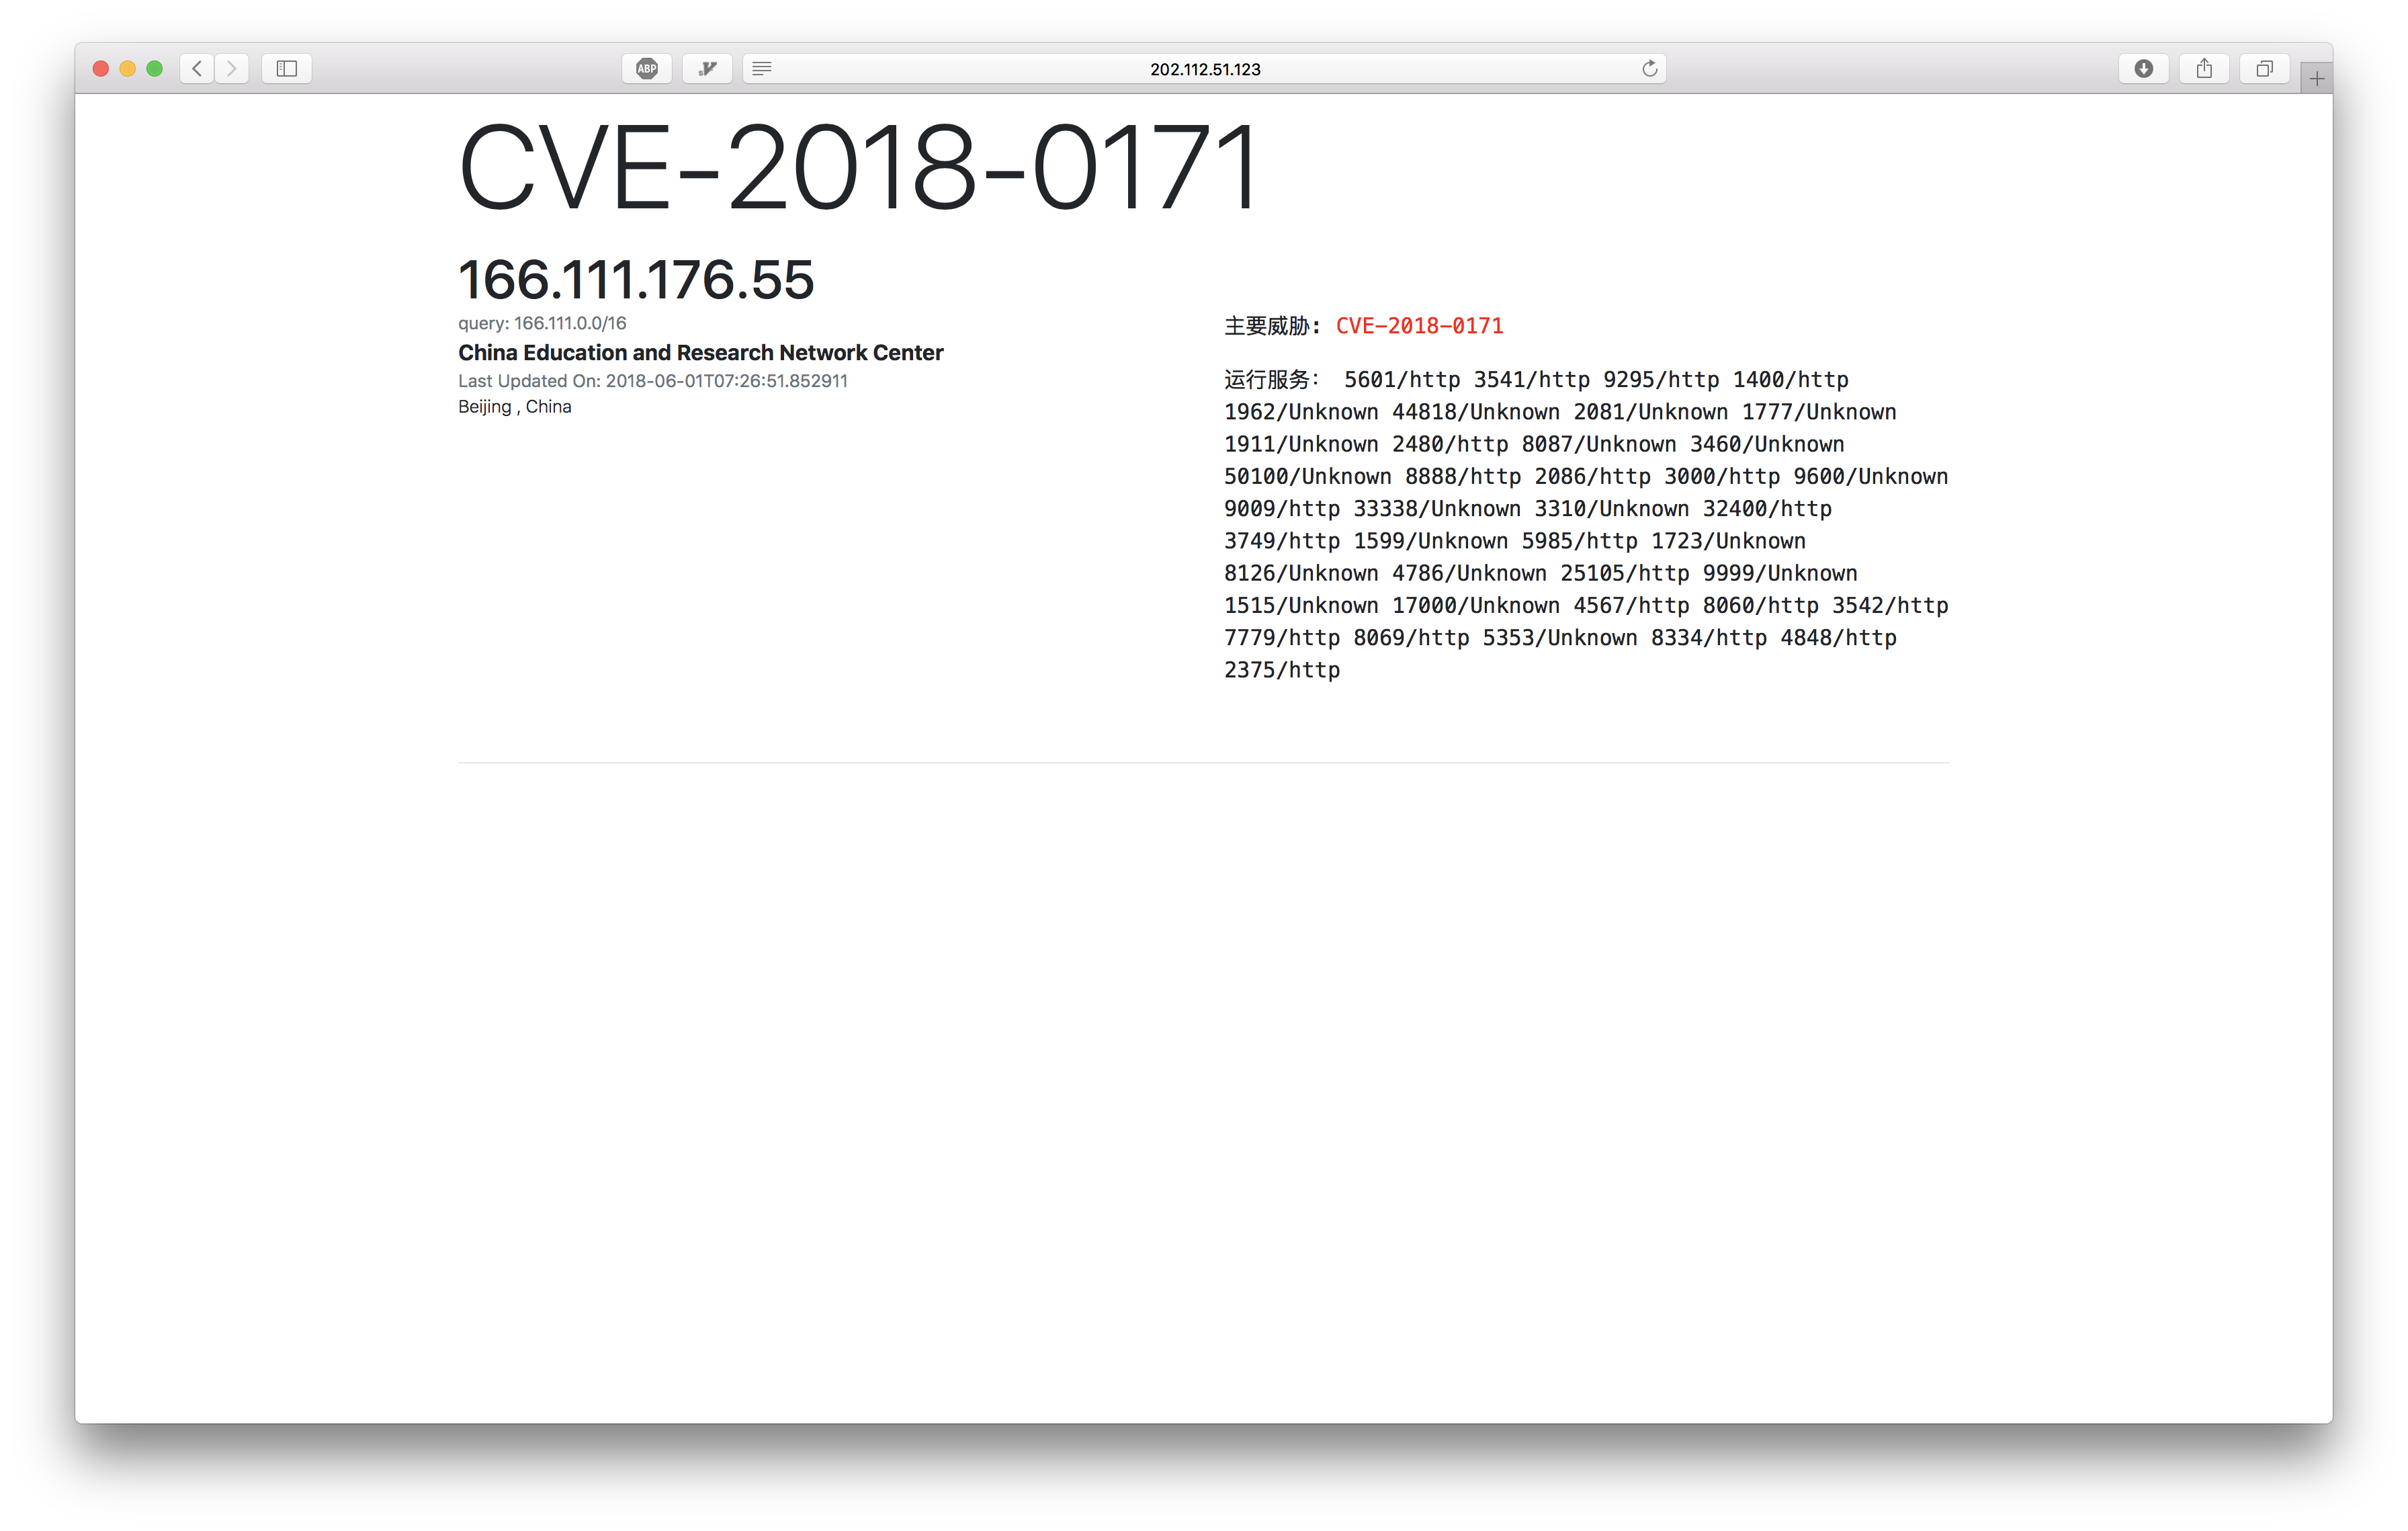
\includegraphics[scale=0.12]{search.png}
    \caption{CVE-2018-0171的搜索结果}
    \label{fig:search}
\end{figure}

作为对比,在Shodan中搜索该CVE,没有结果,表明在此例中系统的聚合和分析功能已经比Shodan具有更多的数据和更强的分析能力。

\subsection{统计功能}
\label{sec:statistics}

点击在首页的左侧的“查看统计数据”可以看到的监测的主机范围内的一些统计数据。图~\ref{fig:statistics}是统计数据的页面。

在页面中我们可以看到在166.111.0.0/16这个范围内开放最多的端口中的5个、运行最多的协议中的5个、可能受到威胁的CVE最多的5个。
值得注意的一点是,这里的统计数据是根据来自3个数据源聚合之后的结果,因此比单个数据源API要更加准确,这是本系统的优势之一。

\begin{figure}[H]
    \centering
    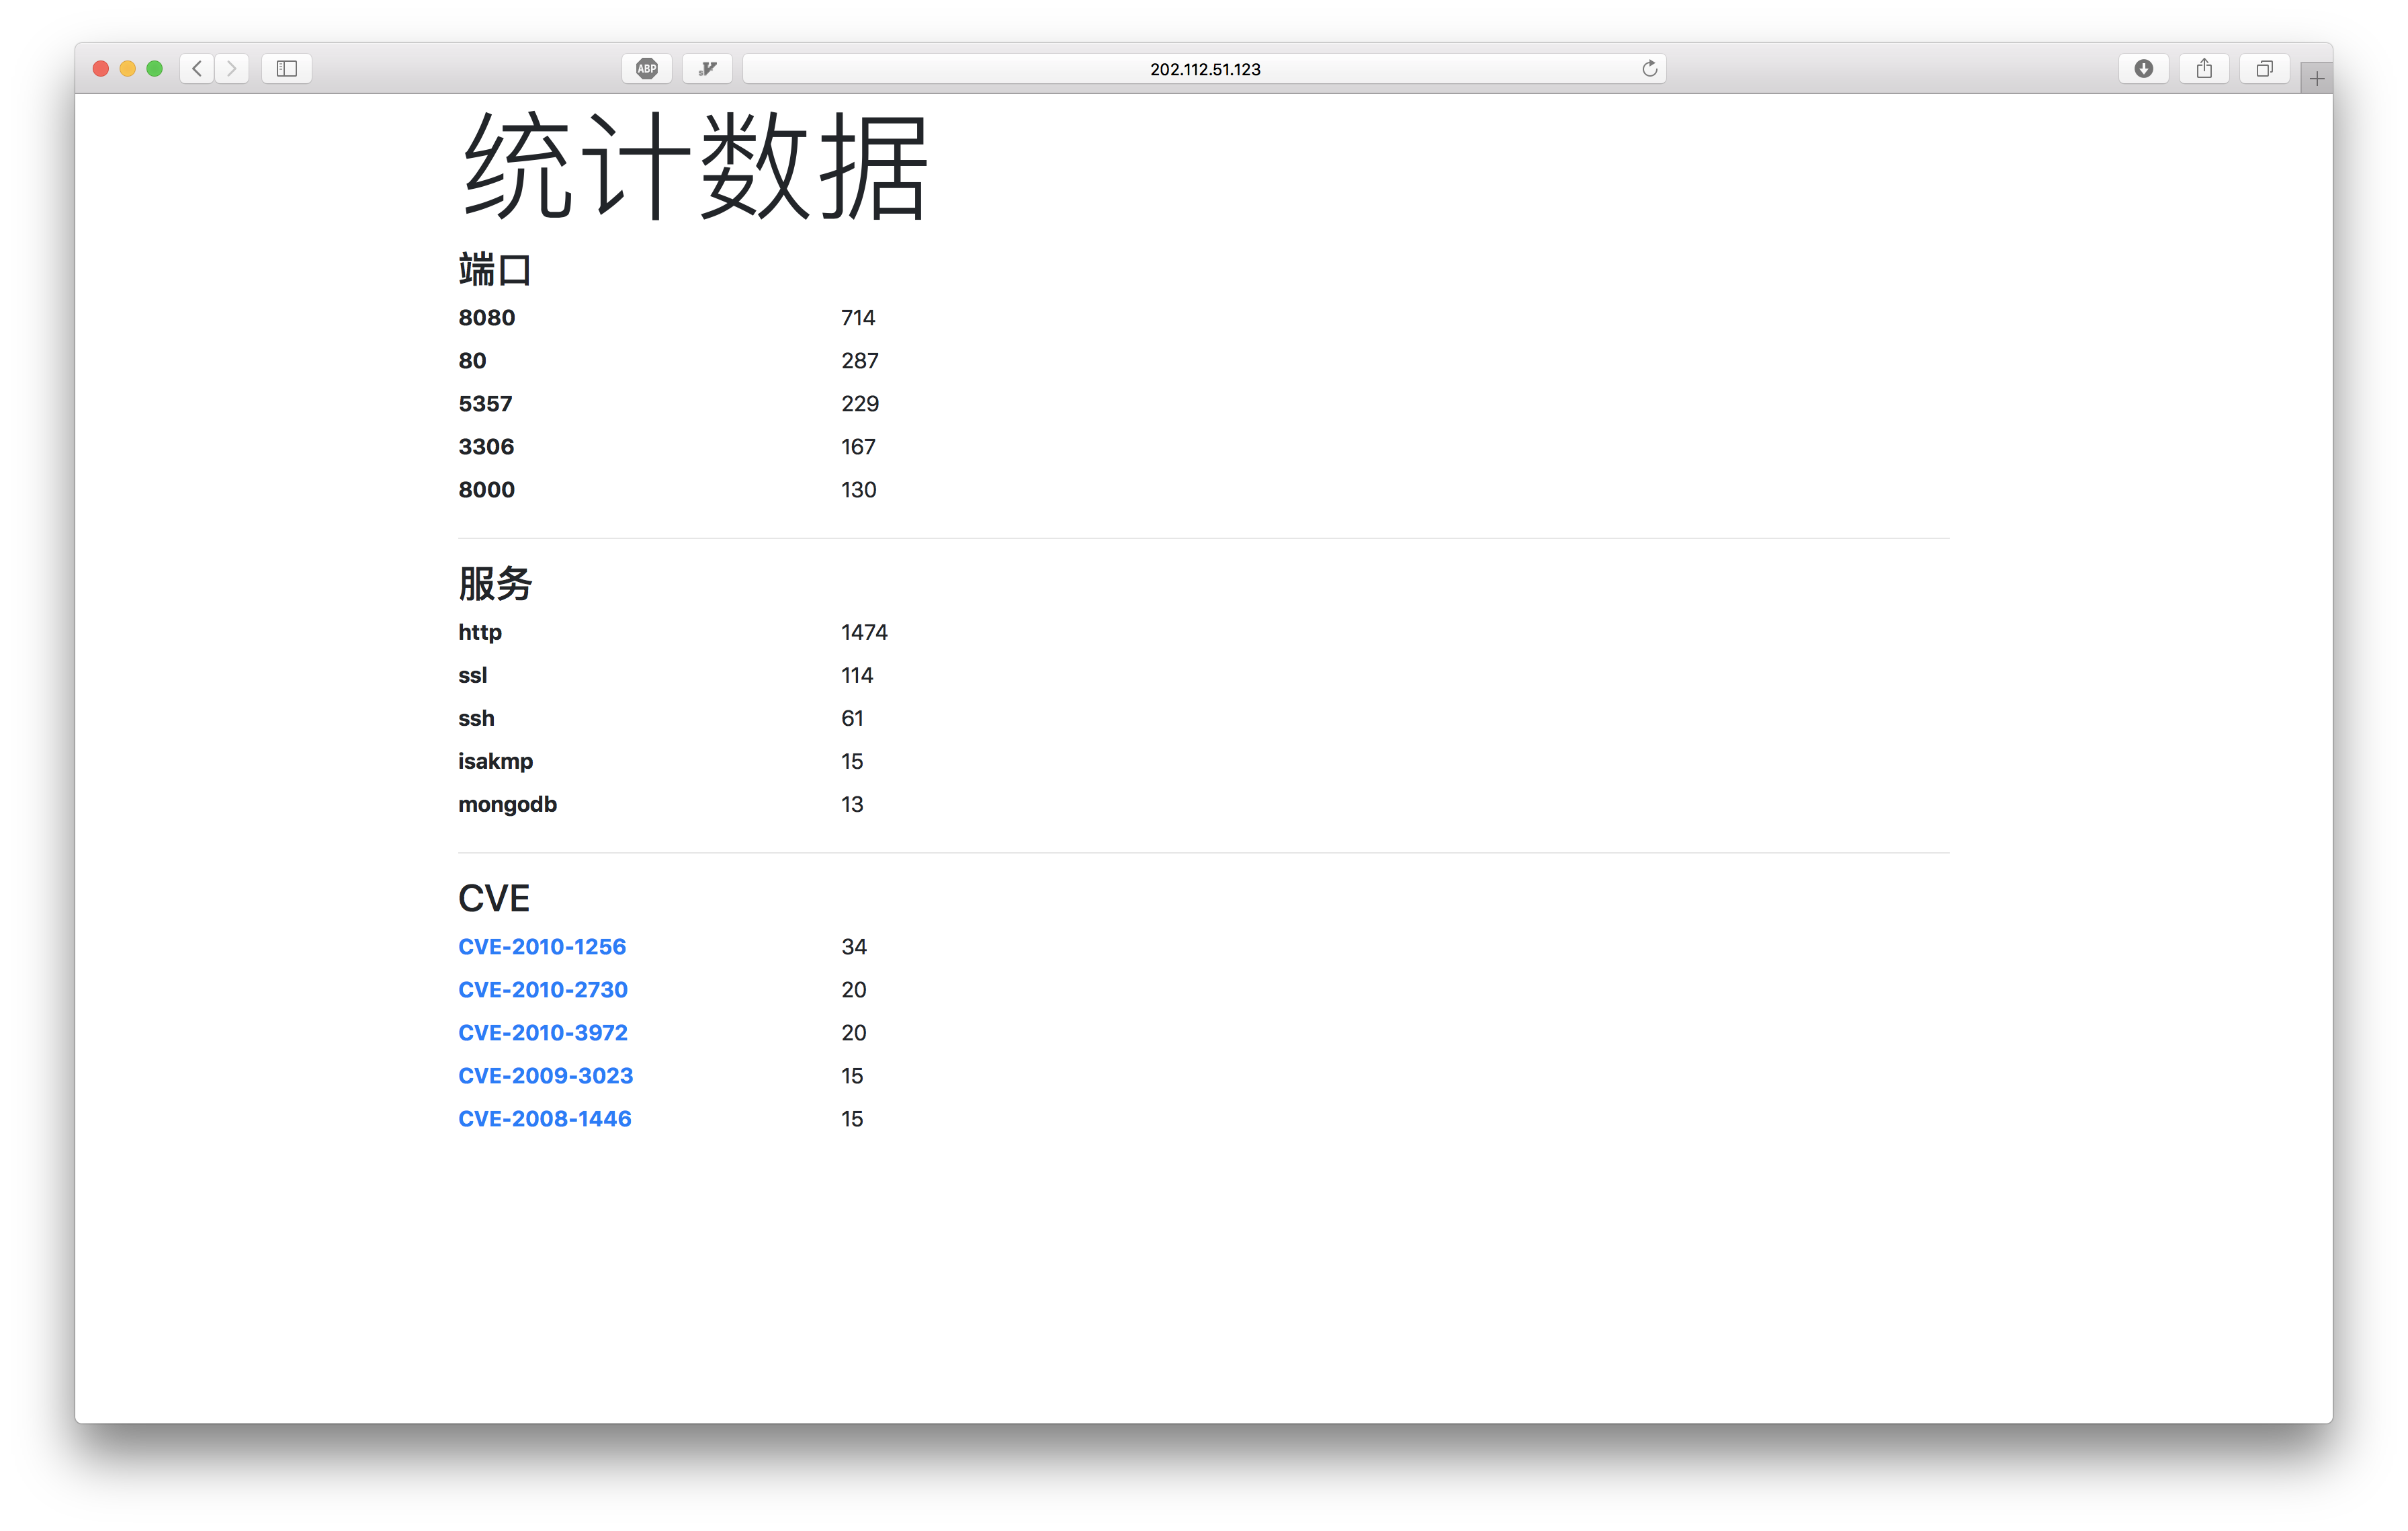
\includegraphics[scale=0.12]{statistics.png}
    \caption{统计数据页面}
    \label{fig:statistics}
\end{figure}

\section{通知}
\label{sec:notification}

本系统的另一个主要特点就是具有推送的功能,这是目前几个搜索引擎都不具备的功能。图~\ref{fig:notification}就是该系统推送后邮箱收到的结果。

\begin{figure}[H]
    \centering
    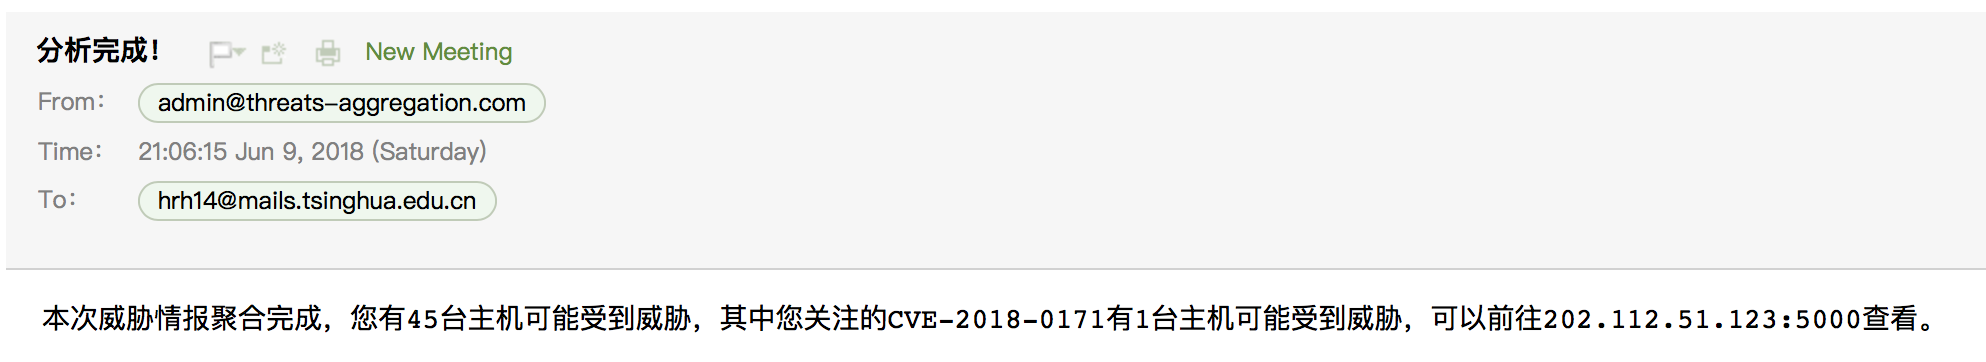
\includegraphics[scale=0.4]{notification.png}
    \caption{系统推送分析结果}
    \label{fig:notification}
\end{figure}

\section{举例验证}
\label{sec:verification}

CVE-2018-0171是一个Cisco发布的利用Smart Install的代码漏洞的远程代码执行严重漏洞,
攻击者可以无需验证就向远端Cisco设备的4786端口发送恶意数据包。采用本系统对该漏洞进行检验。
在图~\ref{fig:search}中我们就能看到搜索该CVE得到的结果,发现有一台主机可能受到该漏洞的威胁。
进入该主机的原始信息里可以看到该主机的“\_shodan”字段的“module”字段为cisco-smi,确实和cisco的IOS软件相关,且开放了4786端口,
该主机的确受到了该CVE的威胁,系统做出的行为正确。图~\ref{fig:verification}即为显示系统显示的界面,点击“查看原始数据”即可找到上述cisco-msi,
验证是否真的受到威胁,或者进一步运行检测脚本进行实际检验。

\begin{figure}[H]
    \centering
    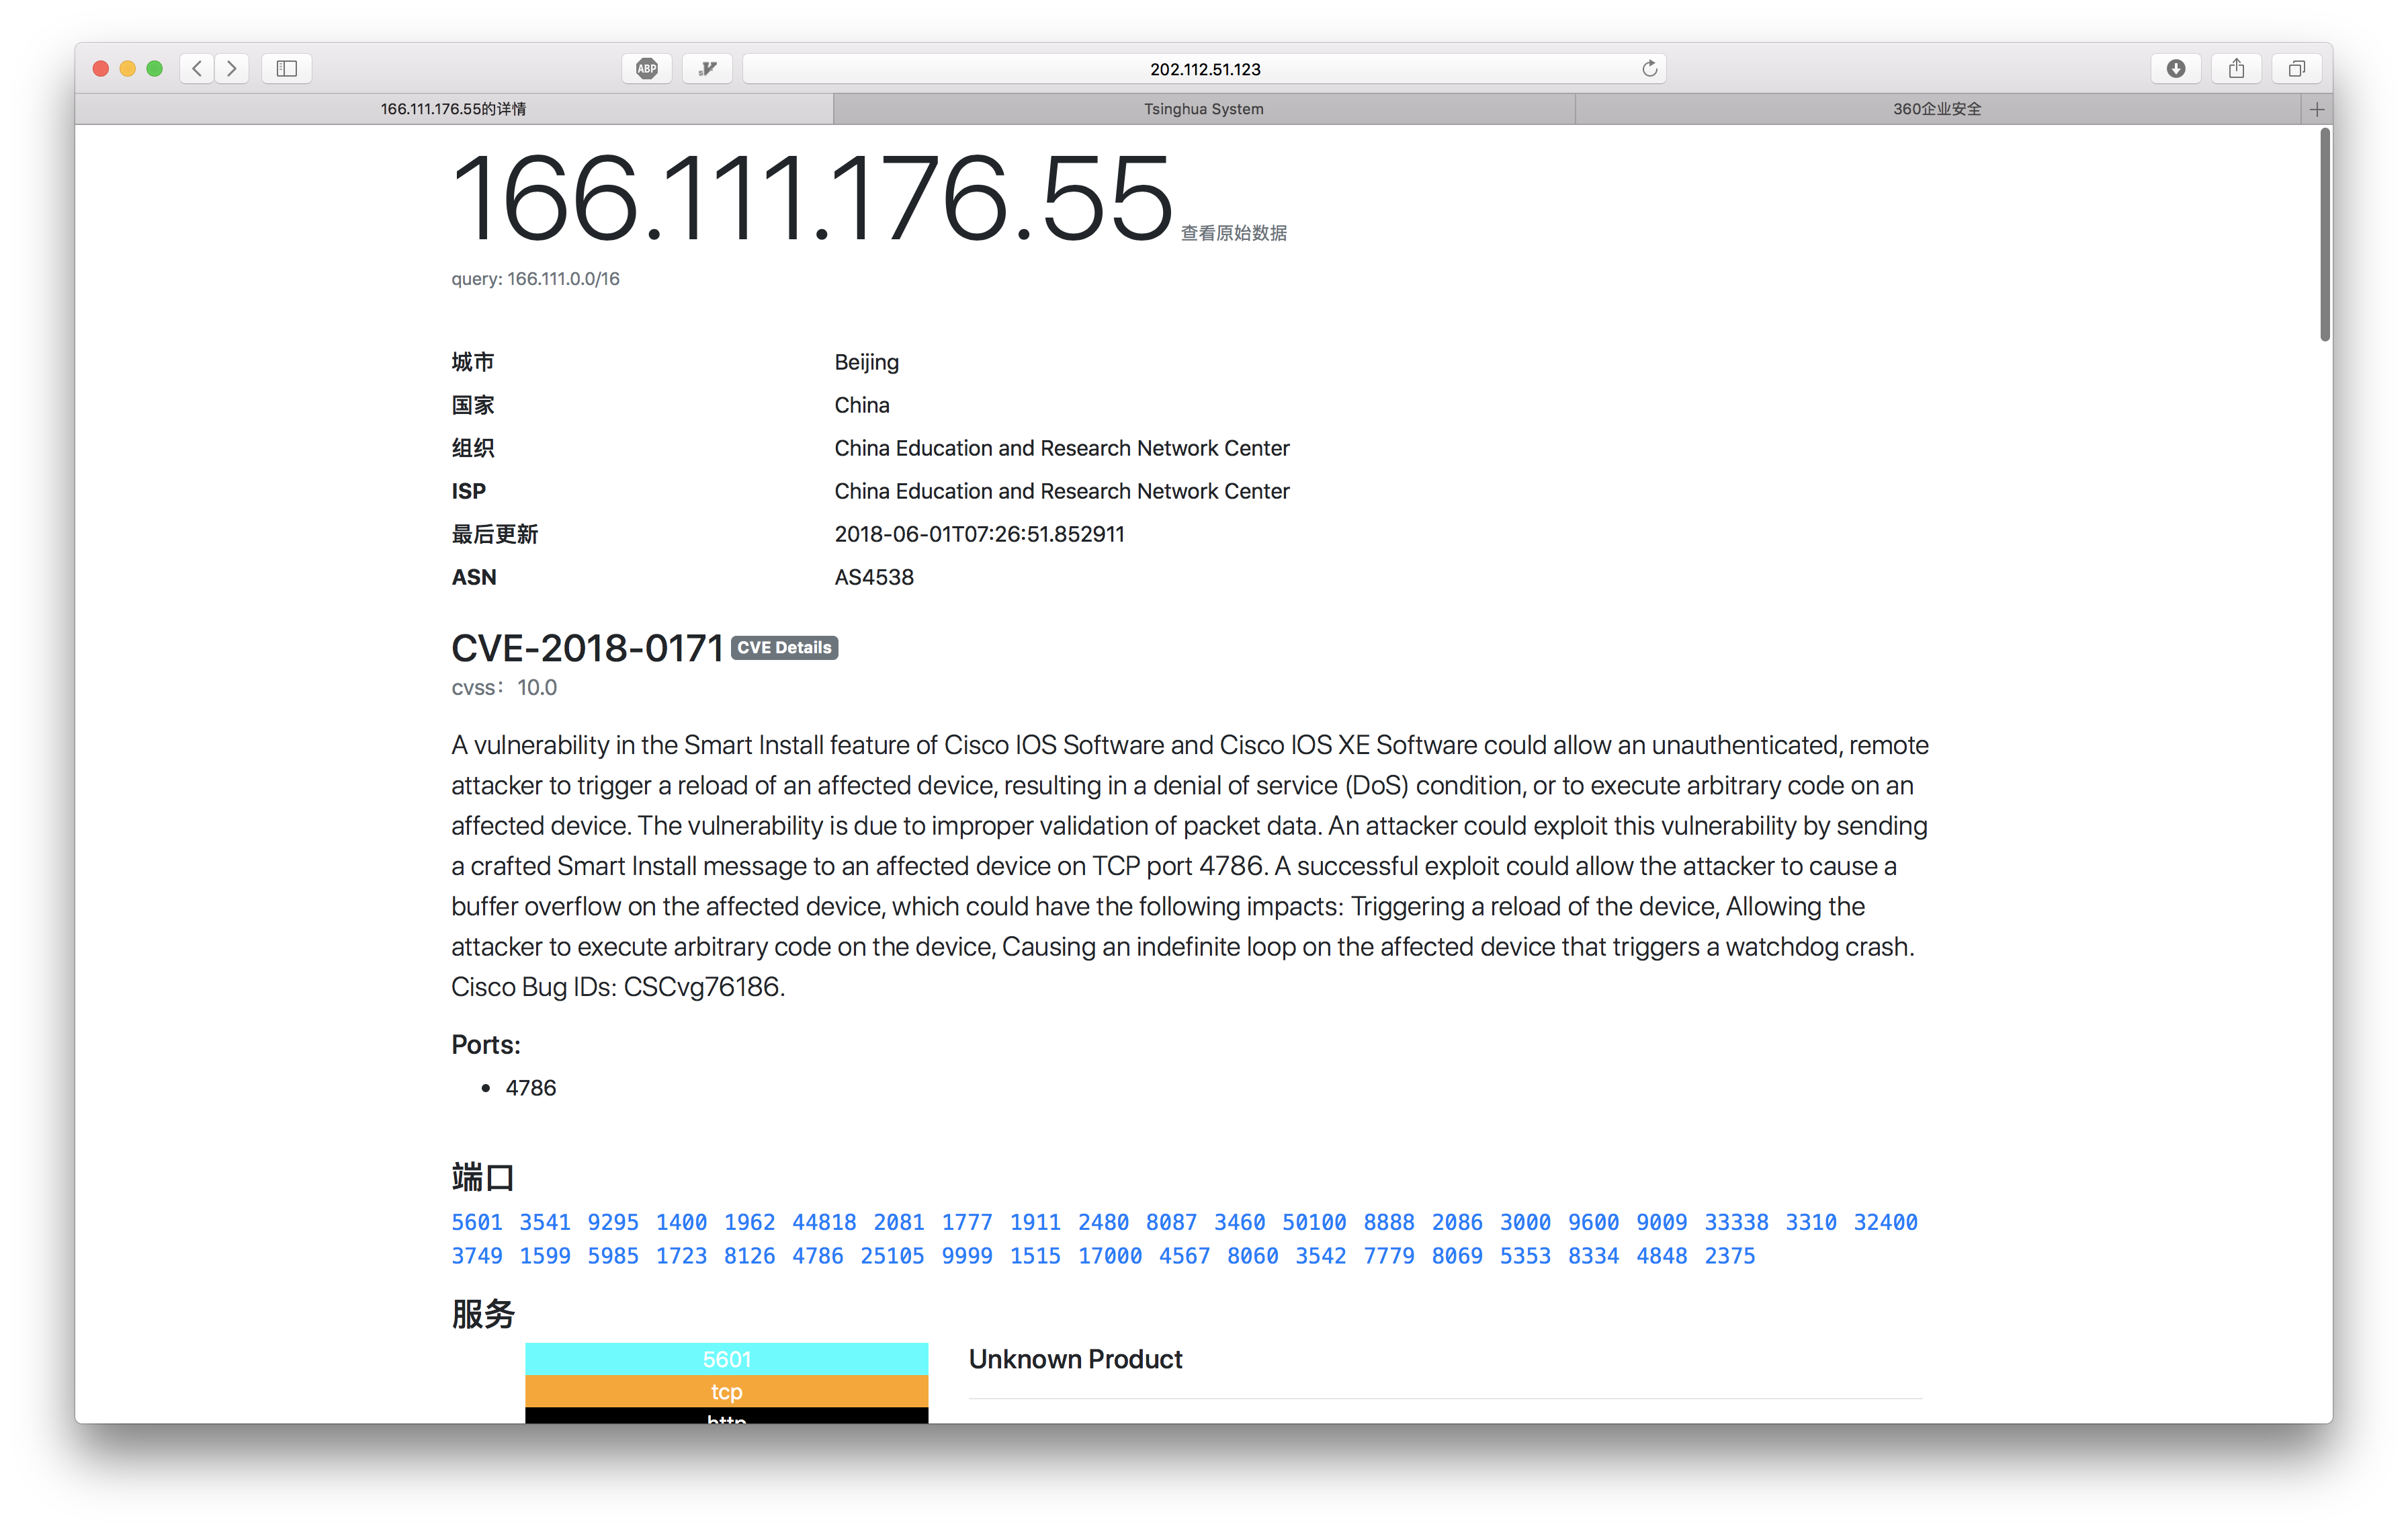
\includegraphics[scale=0.12]{verification.png}
    \caption{可能受到CVE-2018-0171威胁的主机}
    \label{fig:verification}
\end{figure}
